\chapter{End of chapter exercise solutions}

%%%%%%%%%%%%%%%%%%%%%%

\eoceSolCh{Introduction to data}

%%%%%%%%%%%%%%%%%%%%%%

%\begin{multicols}{2}

\eoceSol{(a) Treatment: 60\%. Control: 56\%. (b) There is a 14\% difference in the improvement rates. It appears that patients in the treatment group are more likely to show improvement and, at a first glance, acupuncture appears to be an effective treatment for migraines. (c) It's hard to say. The difference is somewhat large, but the sample is somewhat small.}

\eoceSol{(a) 143,196 eligible subjects who were singletons born between 1989 and 1993. (b) The variables are measurements of CO, NO$_2$, ozone, and particulate matter less than 10?m (PM10) collected at air-quality-monitoring stations as well as the birth weights of the babies. All of these variables are continuous numerical variables. (c) Does air pollution exposure have an effect on preterm births?'}

\eoceSol{(a) 202 black and 504 white men and women who resided in or near New York City, were ages 20-94 years, and had BMIs of 18-35 kg/m$^2$. (b) Age (numerical, continuous), sex (categorical), ethnicity (categorical), weight, height, waist and hip circumference, length of tibia, body density and volume, total body water, body fat percentage, fat free body mass (numerical, continuous). (c) How useful is BMI for predicting body fatness across age, sex and ethnic groups?}

\eoceSol{(a) An observation, i.e. a participant in the survey. (b) 1,691 participants. (c) Gender (gender of the participant), age (age of the participant, in years), maritalStatus (marital status of the participant), grossIncome (gross income of the participant, in $\pounds$, smoke (whether or not the participant smokes), amtWeekends (number of cigarettes smoked on weekend, \# of cigarettes / day), amtWeekdays (number of cigarettes smoked on a week day, \# of cigarettes / day).}

\eoceSol{Gender (categorical), age (numerical, continuous), maritalStatus (categorical), grossIncome (categorical), smoke (categorical), amtWeekends (numerical, discrete), amtWeekdays (numerical, discrete).}

\eoceSol{A horse shoe shaped association - we would expect productivity to increase as stress increases, but up to a point, after that productivity would decrease as stress continued to increase.
\begin{center}
\includegraphics[width = 40mm]{01/figures/eoce/StressProductivity.pdf}
\end{center}
}

\eoceSol{(a) Population mean, $\mu_x = 5.5$; sample mean, $\bar{x} = 6.25$. (b) Population mean, $\mu_x = 52$; sample mean, $\bar{x} = 58$.}

\eoceSol{(a) New average score will be smaller, 73.6. (b) The new score, $x_{25}$, is more than 1 standard deviation away from the previous mean, and this will tend to increase the standard deviation of the data. While possible, it is mathematically rather tedious to calculate the new standard deviation.}

\eoceSol{The distribution of amount of cigarettes smoked on weekends and on weekdays are both right skewed. The values range from 0 to 60 for weekends and from 0 to 55 for weekdays. We can also see that there are more respondents who smoke only a few cigarettes (0 to 5) on the weekdays, about 80 people, than on weekends, about 60 people. Another feature that is visible from the histograms are peaks at 10 and 20 cigarettes. This may be because most people do not keep track of exactly how many cigarettes they smoke, but round their answers to half a pack (10 cigarettes) or a whole pack (20 cigarettes). Due to these peaks the distributions could be classified as bimodal.}

\eoceSol{$s_{amtWeekends} = 0, s_{amtWeekdays} = 4.18$. Variability of the amount of cigarettes smoked is higher on weekdays than on the weekends.}

\eoceSol{(a) 6 (b) 6.5}

\eoceSol{Plot below. \\
\begin{minipage}[c]{0.45\textwidth}
\includegraphics[width = \textwidth]{01/figures/eoce/StatsFinalScoresBoxplot.pdf}
\end{minipage}
}

\eoceSol{(a) The distribution is unimodal and symmetric with a mean around 60. The values range from 50 to 75. This matches the box plot (2) which also shows a symmetric distribution in this range. (b) The distribution is uniform and values range from 0 to 100. This matches box plot (3) which shows a symmetric distribution in this range. Also, each 25\% chunk of the box plot have about the same width and there are no suspected outliers. (c)The distribution is unimodal and right skewed with a median between 1 and 2. The values range from 0 to 7. This matches box plot (1) which also shows a right skewed distribution in this range.}

\eoceSol{(a) Since median is defined as the $50^{th}$ percentile and about 50\% of the data is in the first bar, we would expect median to be between 0 and 20. Q1 is also between 0 and 20 as the $25^{th}$ percentile is in the first bar as well. Q3, defined as the $75^{th}$ percentile, is located between 40 and 60. (b) We would expect the mean to be higher than the median. Since the distribution is right skewed will pull the arithmetic average (mean) up.}

\eoceSol{It appears that marathon times decreased greatly between 1970-1975 and remained somewhat steady after that time for males and females. Males consistently had shorter marathon times than females throughout the years. The data set contains one marathon time for males and one for females each year. These are most probably the winners of each year's marathon. From the box plots of males and females we could tell that males ran faster ``on average" however we could not tell that the winning male time for each year was better than the winning female time. We also could not tell from the histogram or the box plot that marathon times have been decreasing for males and females throughout the years.}

\eoceSol{(a) The distribution is right skewed with potential outliers on the positive end, therefore median and IQR are appropriate measures of center and spread. (b) The distribution is somewhat symmetric and probably does not have outliers, therefore mean and standard deviation appropriate measures of center and spread. (c) The distribution is right skewed. There will be some students who do not consume any alcohol but this is the minimum (there cannot be students who consume fewer than 0 drinks). Most students would consume about the median number of drinks, maybe 2-3 drinks, but there will also be a few students who consume a lot more alcohol than that, giving the distribution a long right tail. Due to the skew, median and IQR are appropriate measures of center and spread. (d) The distribution is right skewed. Most employees will make about the median salary but we would expect to have some high level executives making a lot more, therefore giving the distribution a long right tail. Due to the skew, median and IQR are appropriate measures of center and spread.}

\eoceSol{(a) As well as the order of the categories we can also see the relative frequencies in the bar plot. These proportions are not readily available in the pie chart. (b) None. (c) Bar plot, so that we can also see the relative frequencies of the categories in this graph.}

\eoceSol{(a) Proportion of patients who are alive at the end of the study is higher in the treatment group than in the control group. Therefore survival is not independent of whether or not the patient got a transplant. (b) The shape of the distribution of survival times in both groups is right skewed with outliers on the right side. The median survival time for the control group is much lower than the median survival time for the treatment group, therefore patients who got a transplant typically lived longer. The maximum survival time for the treatment group is much higher (about 5 years) than the maximum survival time for the control group. Even though the maximum survival time for the control group is about 4 years, this observation is an outlier. Overall, very few patients without transplants made it beyond a year while nearly half of the transplant patients survived at least one year. It should also be noted that while the first and third quartiles of the treatment group is higher than those for the control group, the IQR for the treatment group is much bigger, indicating that there is more variability in survival times in the treatment group.}

\eoceSol{(a) The population is all 20-94 year olds. The sample is the 202 black and 504 white men and women who resided in or near New York City and had BMIs of 18-35 kg/m$^2$. (b) The population is all Californians registered to vote in the 2010 midterm elections. The sample is the 1000 registered California voters who were surveyed for this study.}

\eoceSol{(a) This is an observational study. (b) Countries in which a higher percentage of the population have access to the Internet are most probably developed countries which also tend to have a higher quality of life in general and also better health care. Whether or not the country is developed is a lurking variable here, since level of Internet access varies for underdeveloped, developing, and developed countries. (Note: Answers may vary.)}

\eoceSol{(a) Simple random sample. Non-response bias, if only those people who have strong opinions about the survey responds his sample may not be representative of the population. (b) Convenience sample. Under coverage bias, his sample may not be representative of the population since it consists only of his friends.}

\eoceSol{(a) Non-responders are most likely parents who have busier schedules and have difficulty spending time with their kids after school. (b) The women who are not reached 3 years later are most likely renters (as opposed to home owners) who may be from a lower socio economic status. (c) There is no control group and there may be lurking variables. For example, it may be that these people who go running are generally healthier and/or do other exercises.}

\eoceSol{No, this was an observational study. We cannot make such a causal statement based on an observational study. Though the statement is true for this specific sample, it can't be extended to the whole population.}

\eoceSol{(a) Prepare two cups for each participant one containing regular Coke and the other containing Diet Coke. Make sure the cups are identical and contain equal amounts of soda. Label the cups A (regular) and B (diet). (b) Give each participant the two cups, one cup at a time, in random order, and ask the participant to record a value that indicates how much the liked the beverage.  Be sure that neither the participant nor he person handing out the cups knows the identity of the beverage.}

\eoceSol{(a) Experiment. (b) Treatment: exercise twice a week, control: no exercise. (c) Yes, the blocking variable is age. (d) No. (e) Since this is an experiment we can make a causal statement, and since the sample is random the causal statement can be generalized to the population at large.}

\eoceSol{(a) False. Instead of comparing counts, we should compare percentages of people in each group who suffered a heart attack. (b) True. (c) False. Association does not imply causation. We cannot infer a causal relationship based on an observational study. (d) True.}

%\end{multicols}

\noindent\rule{\textwidth}{0.5mm}\vspace{-3mm}
\noindent\rule{\textwidth}{0.5mm}

\addvspace{3mm}

%%%%%%%%%%%%%%%%%%%%%%

\eoceSolCh{Probability}

%\begin{multicols}{2}

\eoceSol{False. The tosses are independent trials.}

\eoceSol{(a) 10 tosses. With a low number of flips the variability in the number of heads observed is much larger, so a result further from 50\% is more likely. (b) 100 tosses. With more flips, the observed proportion of heads would probably be closer to 50\% and therefore above 40\%. (c) 100 tosses. The more flips, the less variability away from 50\%. (d) 10 tosses. Fewer flips mean more volatility and a greater chance of getting far from 50\% and below 30\%.}

\begin{multicols}{2}
\eoceSol{(a) $1/1024$. (b) $1/1024$. (c) $1023/1024$.}

\eoceSol{(a) Figure to the right. (b) 0.05 (c) 0.70 (d) 0.95 (e) 0.05 (f) No, there are bloggers who own both types of cameras.}
%
\noindent
\includegraphics[width=60mm]{02/figures/eoce/psDslrVenn.png}
\end{multicols}

\eoceSol{(a) Yes. (b) Yes. (c) No.)}

\eoceSol{(a) 0.26. (b) 0.23. (c) 0.0598. (d) We assumed that the education level of the husband and wife are independent. This may not be an unreasonable assumption since people often marry people who have a comparable level of education to theirs.}

\eoceSol{(a) Sum greater than 1. (b) OK. (c) Sum less than 1. (d) Negative probabilities make no sense. (e) OK. (f) Probabilities cannot be less than 0 or greater than 1.}

\eoceSol{(a) 0.4236. (b) 0.1458. (c) 0.1875. (d) 0.0625.}

\eoceSol{(a) The distribution is right skewed, with a median between 0 and 50,000. Values range from 0 to 500,000 and there are potential outliers on the higher end. (b) 0.8696. (c) 0.4808. (d) 0.4181. (e) Probably not. It appears that females on average make less money than men, i.e. independence does not hold.}

\eoceSol{No.}

\eoceSol{(a) 0.2825. (b) 0.4167. (c) 0.1905. (d) No, because P(black hair $|$ brown eyes) $\ne$ P(black hair $|$ blue eyes). (Other explanations are possible.)}

\eoceSol{(a) 0.65. (b) 0.72. (c) 0.468. (d) We assumed that the burger preferences of the man and the woman are independent. This may not be a reasonable assumption. (e) 0.514.}

\eoceSol{Female.}

\eoceSol{0.6049.}

\eoceSol{(a) Tree diagram on left below. (b) 0.68. (c) 0.32.}

\eoceSol{(a) Tree diagram on right below. (b) 0.84.}

% FIGURE FOR "Tree diagram below. (b) 0.68. (c) 0.32.
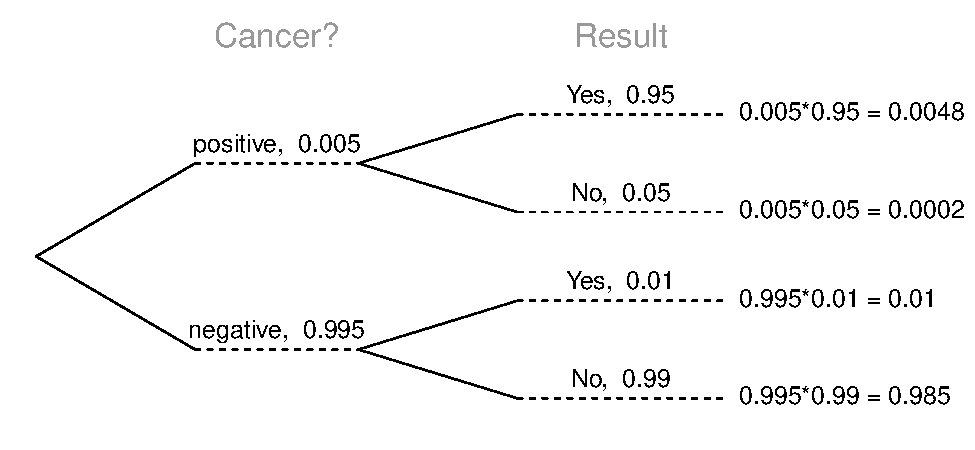
\includegraphics[width=0.4\textwidth]{02/figures/eoce/cancerTree.pdf}
% FIGURE FOR "Tree diagram below (b) 0.84.
\includegraphics[width=0.4\textwidth]{02/figures/eoce/constructBoxPlot.pdf} \vspace{1mm}

\eoceSol{(a) 0.3. (b) 0.3. (c) 0.3. (d) 0.09. (e) No, the draws are independent.}

\eoceSol{(a) 0.091. (b) 0.318. (c) 0.455. (d) 0. (e) 0.288.}

\eoceSol{0.0519.}

\eoceSol{(a) 13. (b) No, this would be unreliable. The students are not a random sample.}

\begin{multicols}{2}
\eoceSol{(a) Table to the right. Expected winnings: \$3.59. (b) EV: -\$1.41, SD: \$3.37. (c) No. The expected net profit is negative so on average you expect to lose money.}
\noindent{\scriptsize\begin{tabular}{llll}
&&&\\
\hline
Event	& 3 hearts & 3 blacks & Else \\
\hline
$X$		& \$50	& \$25	& \$0 \\
$P(X)$	& 0.0129	& 0.1176	& 0.8695 \\
\hline
&&&\\
\end{tabular}}
\end{multicols}

\eoceSol{(a) EV: -\$0.16, SD: \$3. (b) EV: -\$0.16, SD: \$1.73. (c) Expected values are the same but the standard deviations are different. The standard deviation from the game where winnings and losses are tripled is higher, making this game riskier.}

\begin{multicols}{2}
\eoceSol{(a) Table to the right. Expected winnings: -\$0.54 (b) No, he is expected to lose money on average.}
\noindent{\scriptsize\begin{tabular}{lllll}
%&&&&\\
\hline
Event	& 2,...,9	& J, Q, K	& Ace	& A$\clubsuit$ \\
\hline
$X$		& -2		& 1		& 3		& 23 \\
$P(X)$	& 0.6923	& 0.2308	& 0.0577	& 0.0192 \\
\hline
%&&&&\\
\end{tabular}} \vspace{1mm}
\end{multicols}

\eoceSol{\$4.26.}

\eoceSol{(a) Mean: \$3.90, SD: \$0.34. (b) Mean: \$27.30, SD: \$0.89.}

%\end{multicols}

\noindent\rule{\textwidth}{0.5mm}\vspace{-3mm}
\noindent\rule{\textwidth}{0.5mm}

\addvspace{3mm}

%%%%%%%%%%%%%%%%%%%%%%

\eoceSolCh{Distributions of random variables}

%%%%%%%%%%%%%%%%%%%%%%

%\begin{multicols}{2}

\eoceSol{Plots below. (a) 0.09. (b) 0.07. (c) 0.59. (d) 0.05.}
%
\noindent
\includegraphics[width=0.245\textwidth]{03/figures/eoce/zltNeg}
%
\includegraphics[width=0.245\textwidth]{03/figures/eoce/zgtPos}
%
\includegraphics[width=0.245\textwidth]{03/figures/eoce/zBet}
%
\includegraphics[width=0.245\textwidth]{03/figures/eoce/zgtAbs}

\begin{multicols}{2}
\eoceSol{(a) $X \sim N(\mu = 462, \sigma = 119)$, $Y \sim N(\mu = 584, \sigma = 151)$. (b) $Z_{VR} = 1.33$, $Z_{QR} = 0.57$. Plots below. (c) She scored 1.33 standard deviations above the mean on the Verbal Reasoning section and 0.57 standard deviations above the mean on the Quantitative Reasoning section. (d) Perc$_{VR}=91\%$, Perc$_{QR}=72\%$. (e) Verbal Reasoning. (f) VR: 9\%, QR: 28\%. (g) We cannot compare the raw scores since they are on different scales. Comparing her percentiles is more appropriate for determining how well she did compared to others.}
%
\includegraphics[width=50mm]{03/figures/eoce/GRE} \vspace{1mm}
\end{multicols}

\eoceSol{Answers to (b) and (c) would not change, though we would not draw a Normal curve on which to show these scores. We could not answer parts (d) and (e) since the Z table is only valid for the normal model.}

\eoceSol{(a) 711. (b) 400.}

\eoceSol{Figures below. (a) 0.121. (b) 0.156. (c) 62.68 inches. (d) 43.3\%}
%
\noindent
\includegraphics[width=0.24\textwidth]{03/figures/eoce/heightLt48}
%
\includegraphics[width=0.24\textwidth]{03/figures/eoce/heightBet}
%
\includegraphics[width=0.24\textwidth]{03/figures/eoce/heightPerc}
%
\includegraphics[width=0.24\textwidth]{03/figures/eoce/heightLt54}

\eoceSol{(a) 0.140. (b) 70.6$^o$F or colder.}

\eoceSol{(a) 0.68. (b) $x=\$1800$, $\mu=\$1650$. (c) $\sigma=\$220.58$.}

\begin{multicols}{2}
\eoceSol{(a) The book is 1.8 standard deviations above the mean. Usually we say an observation is unusual when it is 2 or more standard deviations from the mean, so this book is not unusually expensive. (b) 0.233. Figure below. (c) If you are following only one auction and set a maximum bid price that is too low, chances are someone will outbid you and you won't win the auction. If your maximum bid price is too high, you may win the auction but you may be paying more than is necessary. If you are following more than one auction and your maximum bid price is too low, chances are you won't win any of the auctions. However if your maximum bid price is too high, you may win more than one auction and end up with multiples of the same item. (d) A reasonable maximum bid would be the cutoff for the cheapest 10\% of auctions. Even though $10^{th}$ percentile is a reasonable cutoff point, we still may end up being too low and not win any auction. (e) Perhaps a little above the $10^{th}$ percentile: \$69.80.}
%
\includegraphics[width=0.3\textwidth]{03/figures/eoce/chemBooks1}
\end{multicols}

\eoceSol{70\% of the data are within 1 SD, 95\% are within 2 SD, and 100\% are within 3 SD of the mean. The data approximately follow the 68-95-99.7\% Rule.}

\eoceSol{The distribution is unimodal, symmetric, approximately follows the 68-95-99.7\% Rule. The superimposed normal curve approximates the distribution reasonably well. Therefore we can say that the distribution is nearly normal. The points on the Normal probability plot also seem to follow a straight line. However there is one outlier on the lower end that is apparent in both graphs.}

\begin{multicols}{2}
\eoceSol{The points on the Normal probability plot seem to follow a straight line, so we can say that the distribution is nearly normal (or at least we don't have convincing evidence that it is not nearly normal).}

\eoceSol{No, in poker cards are dealt without replacement.}

\eoceSol{(a) 0.14. (b) 0.0046. (c) $\mu=6$, $\sigma=5.48$.}

\eoceSol{(a) 0.09. (b) $\mu=10$, $\sigma=9.49$.}

\eoceSol{As $p$ gets smaller, i.e. the event is rare, the expected number of trials before a success and the standard deviation increase.}

% FIGURE FROM "The points on the Normal ...
\includegraphics[width=0.4\textwidth]{03/figures/eoce/QQnorm.pdf}\vspace{1mm}
\end{multicols}

\eoceSol{(a) 0.096. (b) $\mu=8$, $\sigma= 7.48$.}

\eoceSol{(a) Yes, it meets the four required conditions. (b) 0.291. (c) 0.291.}

\eoceSol{(a) $\mu=34.85$, $\sigma=3.25$. (b) Yes, since 45 is more than 3 standard deviations from the mean. (c) 0.0002.}

\eoceSol{(a) 0.167. (b) 0.997.}

\eoceSol{(a) 0.999. (b) 0.246. (c) 0.246. (d) 0 since the other three tosses must be either heads or tails.}

\eoceSol{(a.i) 0.109. (a.ii) 0.218. (b.i) 0.137. (b.ii) 0.449. (b.iii) 0.551. (b.iv) 0.084.}

\eoceSol{The probability model is below.}
{\scriptsize\begin{tabular}{lllll}
\hline
$Y$	& -3	& -1	& 1	& 3 \\
$P(Y)$	& 0.1458	& 0.3936	& 0.3543	& 0.1063 \\
\hline
\end{tabular}} \vspace{1mm}

\eoceSol{(a) 0.0804. (b) 0.0321. (c) 0.0193.}

\eoceSol{(a) Poisson($\lambda=75$). (b) $\mu=\lambda=75$, $\sigma=\sqrt{\lambda} = 8.66$. (c) $Z=\frac{60 - 75}{8.66} = -1.73$. Since 60 customers is within 2 standard deviations of the mean, this would not be considered unusual.}

\eoceSol{$P(X = 70) = \frac{75^{70} e^{-75}}{70!} = 0.0402$}

%\end{multicols}

\noindent\rule{\textwidth}{0.5mm}\vspace{-3mm}
\noindent\rule{\textwidth}{0.5mm}

\addvspace{3mm}

%%%%%%%%%%%%%%%%%%%%%%

\eoceSolCh{Foundations for inference}

%%%%%%%%%%%%%%%%%%%%%%

%\begin{multicols}{2}

\eoceSol{(a) Mean. (b) Mean. (c) Proportion. (d) Mean. (e) Proportion.}

\eoceSol{The point estimates are the corresponding sample values. (a) $\bar{x}=13.65$, median$=14$. (b) $s=1.91$, $IQR_{estimate} = 2$. (c) Use the Z score to evaluate ($Z_{16} = 1.23$, $Z_{18} = 2.28$), so 18 credits is unusually high but 16 is not, where we use 2 as a cutoff for deciding what is unusual.}

\eoceSol{No, sample point estimates only approximate the population parameter, and they vary from one sample to another.}

\eoceSol{(a) Standard error (SE). (b) $SE_{\bar{x}} = \frac{1.91}{\sqrt{100}} = 0.191$}

\eoceSol{(a) $SE_{\bar{x}} = 2.89$ (b) The Z score is 1.73, so this doesn't seem unusually high.}

\eoceSol{(a) Independence is met by the random sampling assumption and that the sample is less than 10\% of the population. The sample size is also sufficiently large. We cannot check the assumption that the distribution isn't extremely skewed. (b) (19.862 , 20.058). (c) We are 90\% confident that the true mean amount of coffee in Starbucks venti cups is between 19.862 ounces and 20.058 ounces. (d) 90\% of random samples of size 50 will yield confidence intervals that capture the true mean amount of coffee in Starbucks venti cups. (e) Yes, 20 ounces is included in the interval. (f) A 95\% confidence interval would be wider. All else kept constant, when confidence level increases so does the margin of error and hence the interval becomes wider.}

\begin{multicols}{2}
\eoceSol{(a) 0.0004 (b) Since the sample is random and the 10\% condition is met, we can assume the that how much one penny weighs is independent of another. Since the population distribution is normal, and hence not extremely skewed, sampling distribution of means will be nearly normal even though $n < 50$. (c) Approximately 0 (d) Plot below. (e) We could not calculate (a) or (b). We could not calculate (a) because we do not have a good enough estimate of standard error. A sample size of 30 is not sufficient to use the Central Limit Theorem. However if in (b) we had a sample size above 50, we could still use the Central Limit Theorem.
\begin{center}
\includegraphics[width=0.4\textwidth]{04/figures/eoce/pennies3}
\end{center} 
 }
 \end{multicols}

\eoceSol{(a) Less. (b) We can infer from the sample statistics that the distribution is skewed, so no we cannot. (c) The only condition that may not be met for normality of the mean relates to skew: it is unclear if the distribution is extremely skewed or not. We'll suppose the skew is strong but not too extreme, something we may like to look into further. Solution: 0.0049. (d) Decreases the standard error by a factor $\sqrt{2}$.}

\eoceSol{When the confidence level increases so does the margin of error and the width of the interval. A wide interval may be undesirable even if the confidence level is higher.}

\eoceSol{(a) False, if we can assume skew is not too extreme. (b) False, we are 100\% sure the average for \emph{these} patients is in this interval. (c) True. (d) False, the confidence interval is not about sample means. (e) False, as the confidence level increases so does the width of the interval. (f) False, since in calculation of the standard error we divide the standard deviation by square root of the sample size.}

\eoceSol{(a) $H_0: \mu = 8$ (On average New Yorkers sleep 8 hrs a night), $H_A: \mu < 8$ (On average New Yorkers sleep less than 8 hrs a night). (b) $H_0: \mu = 15$ (The average amount of company time spent not working is 15 minutes), $H_A: \mu > 15$ (The average amount of company time spent not working is greater than 15 minutes).}

\eoceSol{The hypotheses should be about the population mean ($\mu$), not the sample mean. If he believes that \$1.3 million is an overestimation, the alternative hypothesis should be one-sided. The correct way to set up these hypotheses is as follows: $H_0: \mu = \$1.3~million$, $H_A: \mu < \$1.3~million$.}

\eoceSol{(a) 180 minutes is not in the interval, so this is implausible. (b) 2.2 hours (132 minutes) is in the interval, so we conclude the estimated wait time of 2.2 hours is reasonable. (c) A 99\% confidence interval will be wider than a 95\% confidence interval. Hence even without calculating the interval we can tell that 132 minutes would be in it.}

\eoceSol{(a) $H_0$: Anti-depressants do not work for the treatment of Fibromyalgia. $H_A$: Anti-depressants work for the treatment of Fibromyalgia. (b) Concluding that anti-depressants work for the treatment of Fibromyalgia when they actually do not. (c) Concluding that anti-depressants do not work for the treatment of Fibromyalgia when they actually do. (d) If she makes a Type I error, she will continue taking medication that does not actually treat her disorder. If she makes a Type II error, she will stop taking medication that could treat her disorder.}

\eoceSol{(a) Yes, if we assume there isn't too much skew. (b) $H_0: \mu = 0.25$, $H_A: \mu < 0.25$. $Z=-3.53 \to $ one-sided p-value$=0.0002$. Reject $H_0$: there is sufficient evidence to suggest that the percentage of time college students spend on the Internet for coursework has decreased over the last decade. (c) If the percentage of time college students spend on the Internet for course work has actually remained at 25\%, the probability of getting a random sample of 50 college students where the average percentage of time they spend on the Internet for course work is 10\% or less is 0.0002. (d) Since we rejected $H_0$, it is possible we have made a Type I error.}

\eoceSol{$H_0: \mu = 7$, $H_A: \mu \ne 7$. $Z=-1.04\to$single tail$=0.1492\to$p-value$=2*0.1492=0.2984$. There isn't sufficient evidence to suggest that the average lifespan of all ball bearings produced by this machine is not 7 hours. The manufacturer's claim is not implausible.}

\eoceSol{[RE-EXAMINE THIS EXERCISE] (a) Estimate using the plot: $P(X > 5) = \frac{350 + 100 + 25 + 20 + 5}{3000} = \frac{500}{3000} = 0.17$. (b) Assumptions/conditions are not met. (c) Assumptions/conditions are met. Solution: 0.1788.}

\eoceSol{(a) If the skew is not too strong, the assumptions are met. (b) $H_0: \mu = 432$, $H_A: \mu < 432$. $Z=-3.28 \to$p-value (single tail)$=0.0005$. Since $p-value < \alpha$, reject $H_0$. There is evidence to suggest that the average amount savings of all customers who switch their insurance is less than \$432. (c) Yes, the insurance company's claim may be an overestimate since the hypothesis found evidence to suggest that the average savings is less than the advertised amount. (d) \$376.47 and \$413.54. (e) Yes, the hypothesis test was statistically significant \$432 was not in the confidence interval.}

\eoceSol{(a) The only condition we cannot check is for extreme skew; we will assume this is not an issue. (b) $H_0: \mu = 500$, $H_A: \mu \ne 500$. $Z=-3.86 \to$single tail$\approx 0\to$p-value$\approx 2*0=0$. Since $p-value < \alpha$ (0.05), reject $H_0$. The data provide convincing evidence that the average increase in reading speed is not 500\% (it is below 500\% based on the data). (c) No, the company's claim of an average of 500\% increase in reading speed does not appear to be accurate. (d) 371.88\% to 458.12\%. (e) Yes, the hypothesis test was significant yielding evidence to suggest that the average increase in reading speed was not 500\% and the confidence interval does not contain this amount.}

%\end{multicols}

\noindent\rule{\textwidth}{0.5mm}\vspace{-3mm}
\noindent\rule{\textwidth}{0.5mm}

\addvspace{3mm}

%%%%%%%%%%%%%%%%%%%%%%

\eoceSolCh{Large sample inference}

%%%%%%%%%%%%%%%%%%%%%%

%\begin{multicols}{2}

\eoceSol{(a) Hypothesis test for paired data (b) Independence is satisfied since we have a random sample that is less than 10\% of the population. Normality is satisfied since the sample size is large enough and the two samples are dependent. (c) $H_0: \mu_{diff} = 0$ (There is no difference in average daily high temperature between January 1, 1968 and January 1, 2008), $H_0: \mu_{diff} > 0$ (Average daily high temperature in January 1, 1968 was lower than average daily high temperature in January, 2008.) (d) Z = 1.60, p-value = 0.0548. (e) Fail to reject $H_0$. The data do not provide convincing evidence of temperature warming in the continental US. However it should be noted that the p-value is very close to 0.05. (f) Type II. If we made such an error and concluded that there isn't convincing evidence for temperature warming in the continental US, but in reality average temperature on January 1, 2008 is significantly higher than average temperature on January 1, 1968. (g) Yes.}

\eoceSol{(a) $H_0: \mu_{B} = \mu_{A} \rightarrow \mu_{B} - \mu_{A} = 0$ (The population mean of number of cigarettes smoked per day did not change after the Surgeon General's report), $H_A: \mu_1 > \mu_2 \rightarrow \mu_1 - \mu_2 > 0$ (The population mean of number of cigarettes smoked per day has decreased after the Surgeon General's report) (b) Independence is satisfied since we have a random sample that is less than 10\% of the population. Normality is satisfied since the sample size is large enough and the samples are independent. (c) Z = 1.89, p-value = 0.0294. (d) Reject $H_0$. There is sufficient evidence to suggest that the number of cigarettes smoked per day has decreased after the Surgeon General's report. (e) No, the result of the hypothesis test does not imply causation. (f) Type I.}

\eoceSol{(a) $H_0: \mu_{1990} = \mu_{2004} \rightarrow \mu_{1990} - \mu_{2004} = 0$ (Average math score in 1990 is equal to average math score in 2004), $H_A: \mu_1 > \mu_2 \rightarrow \mu_1 - \mu_2 > 0$ (Average math score in 1990 is different than average math score in 2004) (b) Independence is satisfied since we have a random sample that is less than 10\% of the population. Normality is satisfied since the sample size is large enough and the samples are independent. (c) Z = -1.46, p-value = 0.1442. (d) Fail to reject $H_0$. The data do not provide convincing evidence to suggest that the average score has changed between 1990 and 2004. (e) Type II.}

\eoceSol{(a) $H_0: \mu_M = \mu_W$, $H_A: \mu_M < \mu_W$. Z = -97.35, p-value $\approx$ 0. Reject $H_0$. There is sufficient evidence to suggest that average body fat percentage for women is higher. (b) Women on average tend to weigh less than men. Therefore their lean mass is bound to be lower than that of men.}

\eoceSol{(a) True. (b) False, doubling the sample size would decrease the standard error of the sample proportion only by a factor of $\sqrt{2}$. (c) True. (d) True. (e) False,  success-failure condition is not satisfied therefore the distribution of $\hat{p}$ is not nearly normal.}

\eoceSol{(a) False, a confidence interval is constructed to estimate the population proportion.. (b) True. (c) False, the confidence interval does not tell us what we might expect to see in another random sample. (d) True. (e) True.}

\eoceSol{(a) Sample statistic: proportion of people in the sample who have travelled abroad, $\hat{p} = 0.42$, population parameter: proportion of all students at this university who have travelled abroad, $p$. (b) Independence is satisfied since we have a random sample that is less than 10\% of the population. Normality is satisfied since the success-failure condition is met. (c) (0.34, 0.50) (d) We are 90\% confident that 34\% to 50\% of the students at this university have travelled abroad. (e) 90\% of random samples of 100 would produce a confidence interval that includes the true proportion of students at this university who have travelled abroad.}

\eoceSol{(a) All assumptions/conditions satisfied. (b) We are 95\% confident that 14.5\% to 25.5\% of all students at this university smoke. (c) 385 (d) We are 99\% confident that 73\% to 87\% of all students at this university do not smoke.}

\eoceSol{(a) $H_0: p = 0.35$, $H_A: p > 0.35$. Z = 1.47, p-value = 0.0708. Fail to reject $H_0$. The data do not provide convincing evidence to suggest that the proportion of students at this university who have travelled abroad has increased after the implementation of the study abroad program. (b) If in fact 35\% of students at this university have travelled abroad, the probability of getting a random sample of 100 students where more than 42\% have travelled abroad is 0.0708. (c) Yes.}

\eoceSol{(a) $H_0: p = 0.5$ (50\% of all marketing majors have a double major), $H_A: p > 0.5$ (More than 50\% of all marketing majors have a double major) (b) All assumptions/conditions satisfied. (c) Z = 2.24 (d) 0.025 (e) Reject $H_0$, the data do not provide convincing evidence to suggest that majority of marketing students have a double major.}

\eoceSol{(a) $H_0: p = 0.75$ (75\% of students at this college live at home), $H_A: p > 0.75$ (More than 65\% of students at this college live at home) (b) All assumptions/conditions satisfied. (c) Z = 2.89 (d) If in fact 75\% of student at this college lived at home, the probability of getting a random sample of 400 students where more than 325 live at home would be 0.0019. (e) Reject $H_0$, the data provide convincing evidence to suggest that more than 75\% of students at this college live at home.}

\eoceSol{(a) $H_0: p = 0.50$ (50\% of all independents are oppose the public option plan), $H_A:  p > 0.50$ (More than 50\% of all independents are oppose the public option plan) (b) All assumptions/conditions satisfied.(c) Z = 1.12 (d) If in fact 50\% of all independents oppose the public option plan, the probability of getting a sample of 783 independent where more than 52\% oppose the plan is 0.1314. (e) Fail to reject $H_0$, the data do not provide convincing evidence to suggest that more than half of all independents oppose the public option plan. (f) Yes.}

\eoceSol{$H_0: p = 0.5, H_A: p > 0.5$. All assumptions/conditions satisfied. Z = 2.91, p-value = 0.0018. Reject $H_0$, the data provide convincing evidence to suggest that the rate of correctly identifying a soda for these people is significantly better than just by random guessing.}

\eoceSol{$H_0: p = 0.3, H_A: p > 0.3$. All assumptions/conditions satisfied. Z = 1.89, p-value = 0.0294. Reject $H_0$, the data provide convincing evidence to suggest that the rate of sleep deprivation for New Yorkers is higher than the rate of sleep deprivation in the population at large.}

\eoceSol{(a) $H_0: p = 0.18, H_A: p \ne 0.18$. All assumptions/conditions satisfied. Z = 0.71, p-value = 0.4778. Fail to reject $H_0$, the data do not provide convincing evidence to suggest that the percentage of students at this university who smoke has changed over the last five years. (b) Type II.}

\eoceSol{If in fact the true market share of Dunder Mifflin was 45\%, the probability of getting a sample of 180 businesses where 36\% or more of them have Dunder Mifflin as their sole paper provider would be 0.9925.}

\eoceSol{If in fact 65\% Kansas residents went out of state for college, the probability of getting a sample of 1,500 Kansas residents where more than 1,005 go out of state for college would be 0.0526.}

\eoceSol{If in fact aerocyte is not not associated with a higher risk of stomach cancer, the probability of finding a random sample of 300 individuals where 9\% or more have stomach cancer is 0.0007.}

\eoceSol{Independence is satisfied since both groups are randomly samples and both samples are less than 10\% of the prospective populations. There are at least 10 successes and 10 failures in both samples and the samples are independent of each other. (0.16,0.22) (b) We are 90\% confident that the true proportion of Kansas residents that go out of state for college is 16\% to 22\% higher than the true proportion of California residents who go out of state for college. (c) Yes. (d) No.}

\eoceSol{(a) $H_0: p_D = p_I $ (Proportions of Democrats and independents who support the plan are equal.), $H_0: p_D > p_I $ (Proportion of Democrats who support the plan is higher than the proportion of independents who support the plan.) (b) Z = 11.32 (c) The probability of observing a $z$-statistic of 11.32 or higher given that the proportion of Democrats and independents who support the plan were equal is very low, almost 0. (d) Reject $H_0$, the data provide convincing evidence to suggest that the proportion of Democrats who support the plan is higher than the proportion of independents who support the plan. (e) Type I. (f) No. (g) (0.24, 0.32) (h) We are 90\% confident that the proportion of Democrats who support the plan is between 24\% and 32\% higher than the proportion of Independents who do. (i) 90\% of random samples of equivalent sizes will yield confidence interval that include the true difference between the population proportions of Democrats and Independents who support the plan. (f) No.}

\eoceSol{We are 95\% confident that the proportion of Californians who are sleep deprives is 1.7\% less to 0.1\% more than the proportion of Oregonians who are sleep deprived.}

\eoceSol{(a) False, proportion of males whose favorite color is black is higher than the proportion of females. (b) True. (c) True. (d) True. (e) False, (-0.06,-0.02).}

\eoceSol{(a) $P(Do~not~know | College~Grad) = 0.237, P(Do~not~know | Non~College~Grad) = 0.337$. (b) $H_0: p_{CG} = p_{NCG}, H_A: p_{CG} < p_{NCG}$. (c) Z = -3.18, p-value = 0.0007. (d) Reject $H_0$, the data provide convincing evidence to suggest that the proportion of college graduates who responded do not know is lower than the proportion of non-college graduates who responded do not know.}

\eoceSol{(a) $H_0: p_D = p_R$ (Proportions of Republicans and Democrats who support the use of full-body scans are equal.), $H_0: p_D \ne p_R $ (Proportions of Republicans and Democrats who support the use of full-body scans are different.) (b) Z = 0.68 (c) If in fact the proportions of Republicans and Democrats who support the use of full-body scans at airports were equal, the probability of getting a random sample of 318 Republicans and 318 Democrats where difference between the proportions in these samples is 2\% or higher would be 0.4966. (d) Fail to reject $H_0$, there isn't convincing evidence to suggest that the proportions of Republicans and Democrats who support the use of full-body scans are different. (e) Type II. (f) Yes.}

\eoceSol{(a) $H_0$: The distribution of the format of the book used by the students follows the professor's predictions. $H_A$: The distribution of the format of the book used by the students does not follow the professor's predictions. (b) $E_{hard~copy} = 75.6, E_{print} = 31.5, E_{online} = 18.9$. (c) Independence is satisfied assuming random sampling and since the sample size is less than 10\% of population. All expected counts are at least 10. Format of the book used is a categorical variable. (d) $\chi^2  = 2.32, df = 2, 0.01 < p-value < 0.02$. (e) Reject $H_0$, there is convincing evidence to suggest that the distribution of the format of the book used by the students does not follow the professor's predictions, i.e. the professor seems to be off in her predictions.}

\eoceSol{(a) 47.5 (b) 296.6 (c) 21}

\eoceSol{(a) Table below. (b) $E_K = 875.5, E_C = 729.5$
{\small
\begin{center}
\begin{tabular}{l l c c c}
								&			& \multicolumn{2}{c}{\textit{Went out of state}}	&		\\
\cline{3-4}
								&			& Yes		& No		& Total	\\
\cline{2-5}
\multirow{2}{*}{\textit{State	}}		& Kansas		& 1,005		& 495	& 1,500	\\
								& California	& 600		& 650	& 1,250	\\
\cline{2-5}
								& Total		& 1,605		& 1,145	& 2,750
\end{tabular}
\end{center} 
}
}

\eoceSol{(a) Table below. (b) $H_0$: There is no difference in virologic failure rates between the Nevaripine and Lopinavir groups, $H_A$: There is some difference in virologic failure rates between the Nevaripine and Lopinavir groups. (c) $E_{row~1, col~1} = 18, E_{row~1, col~2} = 102, E_{row~2, col~1} = 18, E_{row~2, col~2} = 102$. (d) Yes. (e) $\chi^2  = 8.37, df = 1, 0.001 < p-value < 0.005$. (f) Reject $H_0$, there is convincing evidence to suggest a difference in virologic failure rates between the Nevaripine and Lopinavir groups, i.e treatment and virologic failure do not appear to be independent.
{\small
\begin{center}
\begin{tabular}{l l c c c}
								&			& \multicolumn{2}{c}{\textit{Virol. failure}}	&		\\
\cline{3-4}
								&			& Yes		& No		& Total	\\
\cline{2-5}
\multirow{2}{*}{\textit{Treatment}}		& Nevaripine	& 26			& 94		& 120	\\
								& Lopinavir	& 10			& 110	& 120	\\
\cline{2-5}
								& Total		& 36			& 204	& 240
\end{tabular}
\end{center} 
}
}

\eoceSol{(a) Table below. (b) $H_0$: There is no difference in rate of quitting smoking between smokers who use a nicotine patch who have and have not been part of a support group., $H_A$: There is some difference in rate of quitting smoking between smokers who use a nicotine patch who have and have not been part of a support group. (c) i. 35 ii. 115 (d) Yes. (e) $\chi^2  = 1.86, df = 1, 0.1 < p-value < 0.2$. Fail to reject $H_0$, the study does not provide convincing evidence to support the claim that being in a support group changes the success rate for quitting smoking when someone is wearing a nicotine patch.
{\small
\begin{center}
\begin{tabular}{l l c c c}
								&			& \multicolumn{2}{c}{\textit{Quitting}}	&		\\
\cline{3-4}
								&			& Quit		& Not quit					& Total	\\
\cline{2-5}
\multirow{2}{*}{\textit{Support}}			& Support		& 40			& 110					& 150	\\
								& No support	& 30			& 120 					& 150	\\
\cline{2-5}
								& Total		& 70			& 230					& 300
\end{tabular}
\end{center}
}
}

\eoceSol{(a) $H_0$: There is no difference in rates of preferred shipping method and age among Los Angeles residents, $H_A$: There is some difference in rates of preferred shipping method and age among Los Angeles residents. (b) Not all expected counts are at least 10. (c) No, not all assumptions are met. See Chapter 6 for an alternative approach to test for independence using this data set.}

%\end{multicols}

\noindent\rule{\textwidth}{0.5mm}\vspace{-3mm}
\noindent\rule{\textwidth}{0.5mm}

\addvspace{3mm}

%%%%%%%%%%%%%%%%%%%%%%

\eoceSolCh{Small sample inference}

%%%%%%%%%%%%%%%%%%%%%%

%\begin{multicols}{2}

\eoceSol{(a) $t^*_{41} = 1.68$ (b) $t^*_{20} = 1.33$ (c) $t^*_{28} = 2.05$ (d) $t^*_{11} = 3.11$}

\eoceSol{With a larger critical value the confidence interval ends up being wider.}

\eoceSol{(a) $H_0: \mu = 8$ (New Yorkers on average sleep 8 hrs per night.), $H_A: \mu < 8$ (New Yorkers on average sleep less than 8 hrs per night.) (b) Independence is satisfied since the sample is random ad less than 10\% of the population. The distribution doesn't appear to be strongly skewed. (c) T = -1.75, df = 24. (d) If in fact the true population mean of the amount New Yorkers sleep per night was 8 hours, the probability of getting a random sample of 25 New Yorkers where the average amount of sleep is 7.73 hrs per night or less is between 0.025 and 0.05. (f) Reject $H_0$, the data provide convincing evidence to suggest that New Yorkers on average sleep less than 8 hours per night. (g) No.}

\eoceSol{(a) We are 90\% confident that New Yorkers on average sleep 7.46 to 7.99 hours per night. (b) Yes.}

\eoceSol{No, a t-test is not appropriate since the distributions of total personal income are extremely skewed.}

\eoceSol{(a) $p-value < 0.005$, Reject $H_0$. (b) $0.01 < p-value < 0.02$, Reject $H_0$. (c) $0.05 < p-value < 0.10$, Fail to reject $H_0$. (d) $p-value < 0.20$, Fail to reject $H_0$.}

\eoceSol{(a) (-0.91, 4.91) (b) We are 95\% confident that those in the group that got the weight loss pill lost 0.91\textit{lbs} less to 4.91\textit{lbs} more than those in the placebo group. (c) No. (d) No.}

\eoceSol{(a) Chicken that were fed linseed on average weigh 218.75 grams while those that were given horsebean weigh on average 160.20 grams. Both distributions are relatively symmetric with no apparent outliers. Weights of chicken that were fed horsebean range from about 100 grams to 225 grams, and weights of chicken that were fed horsebean range from about 150 grams to 300 grams. There is a lot more variability in the weights of chicken that were given linseed. (b) $H_0: \mu_L = \mu_H, H_A: \mu_L \ne \mu_H$. (c) Independence is satisfied since both samples are random and less than 10\% of their prospective populations. The distributions do not appear to be extremely skewed and the samples are independent of each other. (d) $T = 3.02, df = 10, 0.01 < p-value < 0.02$. (e) Reject $H_0$, the data provide convincing evidence to suggest that there is a significant difference between the average weights of chicken that were fed linseed and horsebean. (f) Type I. (g) Yes.}

\eoceSol{(a) $H_0: \mu_A = \mu_M, H_A: \mu_A \ne \mu_M$. $T = 5.46, df = 25,  p-value < 0.01$. Reject $H_0$, the data provide convincing evidence to suggest that there a significant difference between the average fuel efficiency of cars with manual and automatic transmission in terms of their city mileage.}

\eoceSol{We are 95\% confident that cars with manual transmission on average get 5.13 to 10.73 miles per gallon more than cars with automatic transmission.}

\eoceSol{(a) $H_0: p = 0.69, H_A: p < 0.69$. (b) $\hat{p} = 0.57$. (c) The success-failure condition is not satisfied. (d) Each student can be represented with a card. Take 100 cards, 69 black cards representing those who follow the news about Egypt and 31 red cards representing those who do not. Shuffle the cards and draw 30 cards representing the 30 high school students. Calculate the proportion of black cards in this sample, $\hat{p}_{sim}$, i.e. the proportion of those who follow the news. Repeat 10,000 times and plot the resulting sample proportions. The p-value will be the proportion of simulations where $\hat{p}_{sim} \le 0.57$. (e) $p-value = 0.1348$ (Note: Answers may vary.) Fail to reject $H_0$, the data do not provide convincing evidence that the proportion of high school students who followed the news about Egypt is lower than the proportion of American adults who did.}

\eoceSol{(a) $H_0: p_{P} = p_{C}, H_A: p_{P} \ne p_{C}$. (b) -0.35. (c) $p-value = 0.0286$ (Note: Answers may vary.) Reject $H_0$, data provide convincing evidence that people react differently under the two scenarios.}

%\end{multicols}

\noindent\rule{\textwidth}{0.5mm}\vspace{-3mm}
\noindent\rule{\textwidth}{0.5mm}

\addvspace{3mm}

%%%%%%%%%%%%%%%%%%%%%%

\eoceSolCh{Introduction to linear regression}

%%%%%%%%%%%%%%%%%%%%%%

%\begin{multicols}{2}

\eoceSol{(a) The relationship is linear therefore the residuals plot will show randomly distributed residuals around 0. (b) The scatterplot shows a fan shape, with higher variability in $y$ for lower $x$. Therefore the residuals plot will also show a fan shape, wider around lower $x$, narrower around higher $x$.}

\eoceSol{(2) and (5) show a strong correlation. Even though (1) and (4) show a strong association, the relationship is not linear therefore correlation would not be strong. (3) and (6) show very weak or no relationship.}

\eoceSol{(a) Exam 2. (b) Exam 2 and the final are relatively close to each other chronologically, or Exam 2 is probably cumulative so has greater similarities in material to the final exam.}

\eoceSol{(a) 4. (b) 3. (c) 1. (d) 2.}

\eoceSol{(a) The relationship appears to be strong, positive and linear. There appears to be one outlier, a student who is about 63 inches tall whose fastest speed is 0 mph. This is probably a student who doesn't drive. (b) It is unlikely that being tall makes people drive faster. One possible outside factor may be gender. Males tend to be taller than females on average, and they also tend to drive faster. (c) It appears that males are taller on average than females and they also drive faster. The positive association between speed and height appears to be driven by gender.}

\eoceSol{(a) There is a somewhat strong, negative, linear relationship between temperature and crawling age. There is also an outlying month when the average temperature is about 53 \degree F and average crawling age is about 28.5 weeks. (b) Changing the units will not change the form, direction or strength of the relationship between the two variables. After all if higher temperatures measured in \degree F is associated with lower average crawling age measured in weeks, higher temperatures measured in \degree C will be associated with lower average crawling age measured in months. (c) R = -0.70.}

\eoceSol{(a) There is a strong, positive, linear relationship between hip girth and weight. However it should be noted that the relationship is somewhat fan shaped; there is less variability in weights for people with lower hip girth measurements than for people with larger hip girth measurements. The fan shape may be explained by the two groups of people (male and female) apparent in the scatterplot. (b) Changing the units, even if just for one of the variables, will not change the form, direction or strength of the relationship between the two variables.}

\eoceSol{(a) R = 1. (b) R = 1. (c) R = 1.}

\eoceSol{(a) There is a positive, moderately strong, linear association between number of tourists and spending. (b) Explanatory: number of calories,  respons: amount of carbohydrates (in grams). (c) With a regression line we can predict the amount of carbohydrates for a given number of calories. This may be useful information if only calorie counts for the food items are posted but the amount of carbohydrates is not readily available.}

\eoceSol{Even though the relationship appears linear in the scatterplot, there is some possible structure remaining in the residuals, either a fan shape or curvature therefore we should not fit a least squares line to this data.}

\eoceSol{(a) $\widehat{height} =  105.79 + 0.604 * shoulderGirth$. (b) $\hat{b}_1$ = For each centimeter increase in shoulder girth we would expect height to increase on average by 0.604 centimeters. $\hat{b}_0$ = People who have a shoulder girth of 0 cm are expected on average to be 105.79 cm tall. A person with a 0 cm shoulder girth does not make any sense. Here, the $y$-intercept serves only to adjust the height of the line and is meaningless by itself. (c) 166 cm. (d) -6 cm, overestimate. (e) No, extrapolation.}

\eoceSol{44\% of the variation in heights is accounted for by the model, i.e. explained by shoulder girth.}

\eoceSol{No, fan shaped residuals or possible outliers.}

\eoceSol{(a) Influential. (b) Leverage. (c) Neither influential nor leverage.}

\eoceSol{(a) There is a negative, moderately strong, somewhat linear relationship between percent of families who own their home and the percent of the population living in urban areas in 2000. There appears to be one outlier, a state where 100\% of the population is urban. (b) Influential.}

\eoceSol{(a) The relationship appears to be strong, positive and linear. There are a few outliers but no points that appear to be influential. (b) $\widehat{weight} = -105.0113 + 1.0176 * height$ Slope: For each centimeter increase in height, weight is expected to increase on average by 1.0176 kilograms. Intercept: People who are 0 centimeters tall are expected to weigh -105.0113 kilograms. This is obviously not possible. Here, the $y$-intercept serves only to adjust the height of the line and is meaningless by itself. (c) $H_0: b_1 = 0, H_A: b_1 > 0$. The p-value for the two-sided alternative hypothesis ($b_1 \ne 0$) is approximately 0. (Note that this output doesn�t mean the p-value is exactly zero, only that when rounded to four decimal places it is zero.) Therefore the p-value for the one-sided hypothesis will also be very small. Reject $H_0$, height and weight are positively correlated and the true slope parameter is indeed greater than 0.}

\eoceSol{(a) $H_0: b_1 = 0, H_A: b_1 > 0$. P-value for a two-sided alternative hypothesis is approximately 0. Then, the p-value for a one-tailed alternative hypothesis will also be very low. Reject $H_0$, wives' and husbands' heights are positively correlated and the true slope parameter is indeed greater than 0. (b) $\widehat{htWife} = 40.4950 + 0.3310 * htHusband$. (c) Slope: For each additional inch in husband's height, wife's height is expected to increase on average by 0.3310 inches. Intercept: Men who are 0 inches tall are expected to have wives who are on average 40.4950 inches tall. The intercept here is meaningless, it serves only to adjust the height of the line.}

\eoceSol{(a) R = 0.36. (b) 63.334, since $R^2$ is low, the prediction based on this regression model may not be very reliable. (c) No, extrapolation.}

\eoceSol{(a) $\widehat{head~circumference} = 3.91 + 0.78 * 28 = 25.75$. (b) $H_0: b_1 = 0, H_A: b_1 \ne 0$. $T = 2.23, df = 23, 0.02 < p-value < 0.05$. Reject $H_0$,  there is an association between gestational age and head circumference and that the true slope parameter is not 0.}

%\end{multicols}


